%-----------------------------------------------------------------------------%
\chapter{\babTiga}
%-----------------------------------------------------------------------------%
Pada bagian ini akan dijelaskan metodologi yang digunakan dalam penelitian. Metodologi ini mencakup metode implementasi dan metode eksperimen.

\section{Metode Implementasi }
%-----------------------------------------------------------------------------%
Bagian ini menjelaskan bagaimana penulis mengimplementasikan operasi-operasi matriks pada proses \textit{inference} menggunakan OpenCL dan bagaimana penulis mengintegrasikan hasil implementasi tersebut ke Tensorflow Lite sehingga dapat digunakan oleh Tensorflow Lite ketika melakukan proses \textit{inference}.

\subsection{Metode Implementasi Konvolusi Matriks }
Operasi konvolusi matriks melibatkan tiga buah matriks yaitu matriks masukan, matriks filter, dan matriks keluaran. Matriks-matriks tersebut merupakan matriks empat dimensi yaitu kanal, baris, kolom, dan \textit{batch}. Seluruh matriks masukan dan keluaran disimpan di memori GPU secara linear dengan struktur seperti contoh pada \pic~\ref{fig:linearconv}. Pada contoh tersebut, elemen ke-15 dari data linear adalah elemen pada kanal ke-7, kolom ke-2, baris ke-1 dan \textit{batch} ke-1 dari matriks. Semua matriks menggunakan tipe data vektor $float4$. Apabila banyaknya kanal dari matriks bukan kelipatan empat, maka diberikan \textit{padding} pada struktur linear di memori GPU tersebut sedemikian sehingga setiap vektor $float4$ mengandung elemen-elemen yang merupakan elemen-elemen matriks pada kolom, baris, dan \textit{batch} yang sama.

\begin{figure}
	\centering
	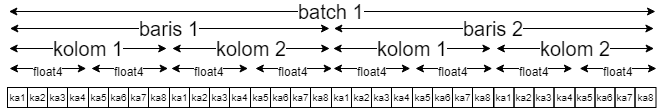
\includegraphics[width=0.75\textwidth]
	{pics/linearconv.png}
	\caption{Contoh struktur linear matriks masukan, matriks filter, dan keluaran yang disimpan di memori GPU untuk operasi konvolusi.}
	\label{fig:linearconv}
\end{figure}

Misalkan ukuran $tinggi \times lebar \times kanal \times \textit{batch}$ dari matriks masukan, matriks filter, dan matriks keluaran berturut-turut adalah $H_i \times W_i \times C_i \times B_i$, $H_f \times W_f \times C_f \times B_f$, dan $H_o \times W_o \times C_o \times B_o$. Pada implementasi ini digunakan \textit{NDRange} dua dimensi berukuran $H_{ws} \times W_{ws}$ dan \textit{work-group} dua dimensi berukuran $H_{wg} \times W_{wg}$ dengan $H_{ws} = H_o' \times B_o$ dan $W_{ws} = W_o' \times ceil(C_o/4)$, dimana $Wo'$ adalah bilangan kelipatan $W_{wg}$ terkecil yang lebih besar atau sama dengan $W_o$ dan $H_o'$ adalah bilangan kelipatan $H_{wg}$ terkecil yang lebih besar atau sama dengan $H_o$. \pic~\ref{fig:wiconv} merupakan contoh struktur \textit{NDRange} dengan $H_{wg} = 8$ dan $W_{wg} = 32$.

\begin{figure}
	\centering
	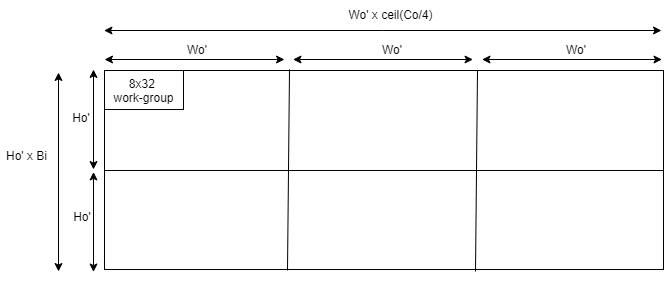
\includegraphics[width=0.75\textwidth]
	{pics/wiconv.png}
	\caption{Contoh struktur \textit{NDRange} untuk operasi konvolusi matriks.}
	\label{fig:wiconv}
\end{figure}

Dengan struktur tersebut, setiap vektor $float4$ pada matriks keluaran dikomputasi oleh suatu \textit{work-item} yang unik. Selain itu, suatu \textit{work-group} melakukan komputasi untuk memperoleh satu blok matriks keluaran dengan ukuran $kanal \times tinggi \times lebar = 4 \times H_{wg} \times W_{wg}$. Blok tersebut merupakan hasil konvolusi dari suatu blok lain pada matriks masukan dengan ukuran $kanal \times tinggi \times lebar = C_i \times (H_{wg}+H_f-1) \times (W_{wg}+W_f-1)$ dengan empat matriks filter yang berbeda. Ini dapat dilihat pada \pic~\ref{fig:convblock}.   

\begin{figure}
	\centering
	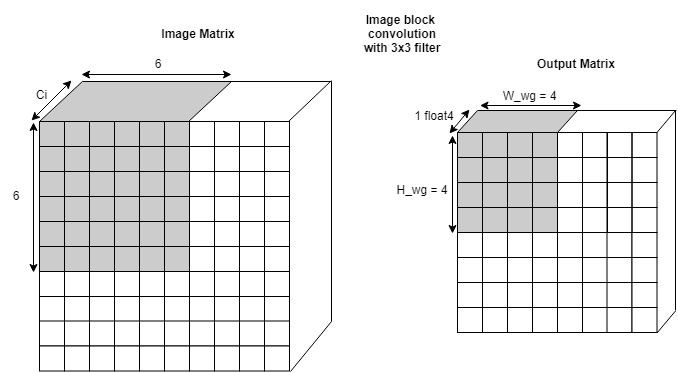
\includegraphics[width=0.75\textwidth]
	{pics/convblock.png}
	\caption{Blok pada matriks keluaran (berwarna abu-abu) yang merupakan hasil konvolusi dari blok (berwarna abu-abu) pada matriks masukan yang dikomputasi oleh suatu \textit{work-group}.}
	\label{fig:convblock}
\end{figure}

Perhatikan bahwa untuk memperoleh satu blok matriks keluaran, hampir semua elemen pada blok matriks masukan akan diakses lebih dari satu kali oleh \textit{work-group}. Mengetahui fakta ini, penulis menggunakan \textit{local memory caching} untuk mengurangi redundansi akses ke memori global. Konvolusi untuk suatu blok matriks keluaran dilakukan dalam $ceil(C_i/4)$ iterasi, dimana setiap iterasi hanya melibatkan blok matriks masukan yang berukuran $kanal \times tinggi \times lebar = 4 \times (H_{wg}+H_f-1) \times (W_{wg}+W_f-1)$ seperti yang dapat dilihat pada \pic~\ref{fig:conviter}. Hasil konvolusi dari semua iterasi kemudian diakumulasikan. Dengan menggunakan \textit{local memory caching}, pada setiap iterasi blok matriks masukan ini disalin terlebih dahulu dari memori global ke memori lokal sebelum digunakan untuk komputasi. Setiap \textit{work-item} pada \textit{work-group} bertugas menyalin maksimal empat vektor $float4$ dari blok matriks masukan ke memori lokal seperti yang terlihat pada \pic~\ref{fig:convlocal}.  

\begin{figure}
	\centering
	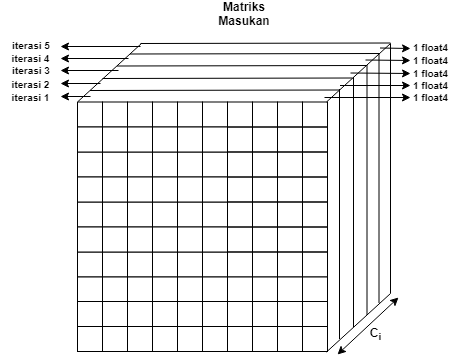
\includegraphics[width=0.75\textwidth]
	{pics/conviter.png}
	\caption{Operasi konvolusi yang dilakukan dalam $ceil(C_i/4)$ iterasi dimana $C_i$ adalah kedalaman matriks masukan.}
	\label{fig:conviter}
\end{figure}

\begin{figure}
	\centering
	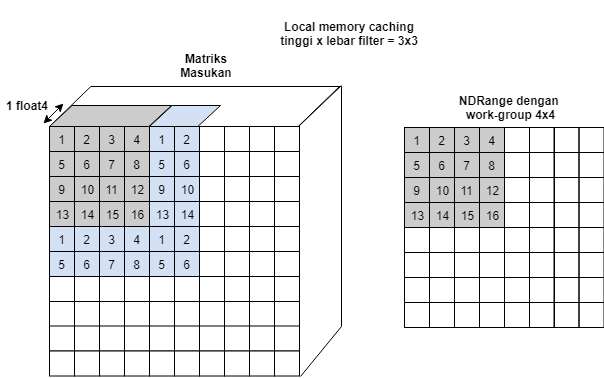
\includegraphics[width=0.75\textwidth]
	{pics/convlocal.png}
	\caption{Contoh \textit{local memory caching} terhadap matriks masukan pada suatu iterasi dimana \textit{work-item} dengan nomor $i$ bertugas menyalin vektor-vektor $float4$ dari matriks masukan dengan nomor $i$ ke memori lokal.}
	\label{fig:convlocal}
\end{figure}

Selain melakukan \textit{local memory caching} terhadap blok pada matriks masukan, \textit{local memory caching} juga dilakukan terhadap blok matriks filter. Blok matriks filter yang dimaksud adalah blok pada matriks filter yang dikalikan titik dengan blok matriks masukan yang telah disimpan di memori lokal. Blok ini berukuran $kanal \times tinggi \times lebar = 4 \times H_f \times W_f$. Untuk menghasilkan suatu kanal pada matriks keluaran, semua \textit{work-item} pada \textit{work-group} menggunakan blok matriks filter yang sama. Karena suatu \textit{work-group} memproses blok matriks keluaran dengan kanal sebanyak empat, maka pada setiap iterasi \textit{caching} dilakukan terhadap empat blok matriks filter yang berbeda seperti yang terlihat pada \pic~\ref{fig:convlocalfilter}. Setiap \textit{work-item} pada \textit{work-group} bertugas menyalin maksimal empat vektor $float4$ dari matriks filter yang berada di memori global ke memori lokal.

\begin{figure}
	\centering
	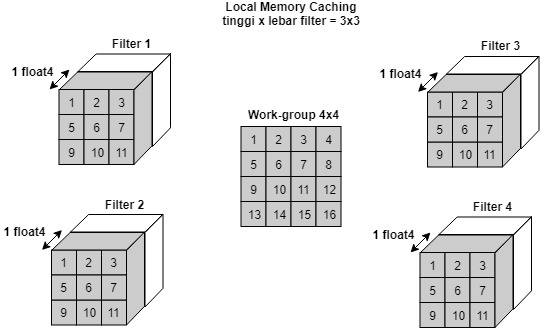
\includegraphics[width=0.75\textwidth]
	{pics/convlocalfilter.png}
	\caption{Contoh \textit{local memory caching} terhadap blok matriks filter yang terkait dengan blok matriks masukan pada suatu iterasi, dimana \textit{work-item} dengan nomor $i$ bertugas menyalin vektor-vektor $float4$ dari matriks filter dengan nomor $i$ ke memori lokal.}
	\label{fig:convlocalfilter}
\end{figure}

Perhatikan bahwa penggunaan metode \textit{local memory caching} seperti yang telah dijelaskan di atas mewajibkan ukuran $tinggi \times lebar$ dari \textit{work-group} harus sama dengan atau lebih besar dari ukuran $tinggi \times lebar$ dari matriks filter.

\subsection{Metode Implementasi Perkalian Matriks-Matriks }
Dalam pembahasan ini dimisalkan matriks masukan adalah matriks A dan matriks B, sedangkan matriks keluaran adalah matriks C. Sama seperti konvolusi, seluruh matriks disimpan secara linear di memori GPU. Matrix A dan matriks C disimpan secara \textit{row-major}, sedangkan matrix B disimpan secara \textit{column-major} seperti pada \pic~\ref{fig:linearmatmat}.  Semua matriks menggunakan tipe data vektor $float4$. Jika lebar dari matriks A atau C bukan kelipatan 4, maka diberikan \textit{padding} pada struktur linear di memori GPU sedemikian sehingga setiap vektor $float4$ mengandung elemen-elemen yang merupakan elemen-elemen matriks pada baris yang sama. Untuk matriks B, \textit{padding} diberikan jika tingginya bukan kelipatan 4.

\begin{figure}
	\centering
	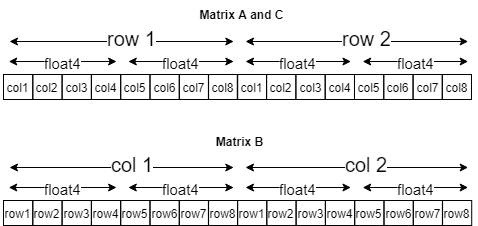
\includegraphics[width=0.75\textwidth]
	{pics/linearmatmat.png}
	\caption{Contoh struktur linear matriks A, B, dan C pada operasi perkalian matriks-matriks.}
	\label{fig:linearmatmat}
\end{figure}

Misalkan ukuran $tinggi \times lebar$ dari matriks A adalah $M \times K$ sedangkan matriks B adalah $K \times N$, maka matriks C berukuran $M \times N$. Untuk menjalankan operasi perkalian matriks-matriks di GPU, digunakan \textit{NDRange} dua dimensi dengan ukuran $H_{ws} \times W_{ws}$ dan \textit{work-group} dua dimensi berukuran $H_{wg} \times W_{wg}$ dimana $H_{ws}$ adalah bilangan kelipatan $H_{wg}$ terkecil yang lebih besar atau sama dengan $M$ dan $W_{ws}$ adalah bilangan kelipatan $W_{wg}$ terkecil yang lebih besar atau sama dengan $ceil(N/4)$. Untuk ukuran \textit{work-group}, berlaku aturan $H_{wg} = 4 \times W_{wg}$. 

\begin{figure}
	\centering
	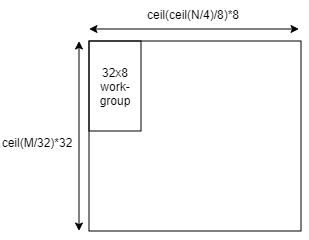
\includegraphics[width=0.75\textwidth]
	{pics/wimatmat.png}
	\caption{Contoh struktur \textit{NDRange} untuk perkalian matriks-matriks.}
	\label{fig:wimatmat}
\end{figure}

Dengan struktur di atas, setiap vektor $float4$ pada matriks C dikomputasi oleh satu \textit{work-item} yang unik. Lalu, masing-masing \textit{work-group} melakukan komputasi untuk memperoleh satu blok pada matriks C yang berukuran $H_{wg} \times H_{wg}$ seperti pada \pic~\ref{fig:wimatmat}. Perhatikan bahwa setiap blok matriks C tersebut diperoleh dari perkalian matriks antara dua blok lain, yaitu satu blok dari matriks A berukuran $H_{wg} \times K$ dan satu blok dari matriks B berukuran $K \times H_{wg}$. \pic~\ref{fig:blackmatmat} adalah contoh perkalian antara dua blok matriks untuk menghasilkan blok berukuran $32 \times 32$ pada matriks C ketika ukuran \textit{work-group} adalah $32 \times 8$.

\begin{figure}
	\centering
	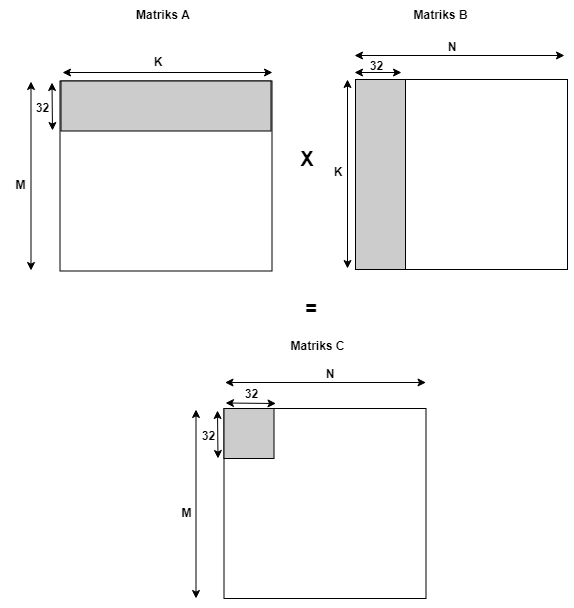
\includegraphics[width=0.75\textwidth]
	{pics/blockmatmat.png}
	\caption{Perkalian antara dua blok berukuran $32 \times K$ dan $K \times 32$ pada matriks A dan matriks B sehingga menghasilkan satu blok berukuran $32 \times 32$ pada matriks C.}
	\label{fig:blockmatmat}
\end{figure}

Seperti pada konvolusi, perkalian dua blok matriks tersebut juga mengandung redundansi akses terhadap memori global karena elemen-elemen yang sama pada blok diakses lebih dari satu kali dalam suatu \textit{work-group}. Penulis juga menggunakan metode \textit{local memory caching} dalam implementasi ini. Perkalian antar dua blok matriks A dan B dilakukan dalam $ceil(K/H_{wg})$ iterasi. Pada setiap iterasi, dilakukan perkalian dua blok yang berukuran lebih kecil yaitu antara blok $H_{wg} \times H_{wg}$ dari matriks A dengan blok $H_{wg} \times H_{wg}$ dari matriks B seperti pada \pic~\ref{fig:matmatiter}. Hasil perkalian dari semua iterasi kemudian diakumulasikan. Pada setiap iterasi, masing-masing \textit{work-item} pada \textit{work-group} berutgas menyalin dua vektor $float4$, satu dari blok matriks A dan satu dari blok matriks B, ke memori lokal seperti yang terlihat pada \pic~\ref{fig:localmatmat} sebelum komputasi dilakukan.

\begin{figure}
	\centering
	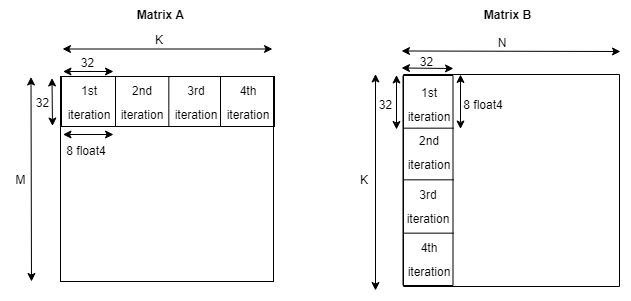
\includegraphics[width=0.75\textwidth]
	{pics/matmatiter.png}
	\caption{Operasi perklaian matriks-matriks yang dilakukan dalam $ceil(K/32)$ iterasi dimana setiap iterasi melibatkan blok matriks A dengan lebar 32 dan blok matriks B dengan tinggi 32.}
	\label{fig:matmatiter}
\end{figure}

\begin{figure}
	\centering
	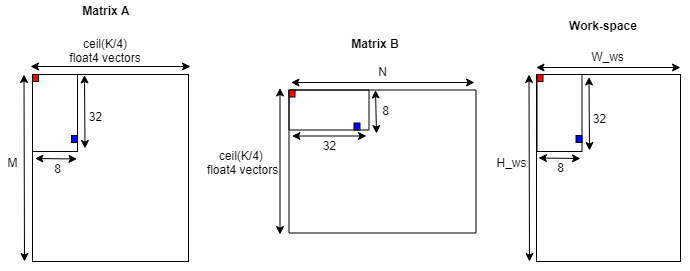
\includegraphics[width=0.75\textwidth]
	{pics/localmatmat.png}
	\caption{Contoh \textit{local memory caching} pada perkalian matriks-matriks, dimana masing-masing \textit{work-item} menyalin dua vektor $float4$ (\textit{work-item} merah memuat vektor berwarna merah dan \textit{work-item} biru memuat vektor berwarna biru).}
	\label{fig:localmatmat}
\end{figure}

\subsection{Metode Integrasi OpenCL \textit{Kernel} ke Tensorflow Lite }
%-----------------------------------------------------------------------------%
Pada penelitian ini penulis memanfaatkan Tensorflow Lite untuk menjalankan proses \textit{inference} pada \textit{Deep Learning} pada perangkat \textit{mobile}. Penulis memodifikasi kode sumber Tensorflow Lite dengan menambahkan \textit{kernel} untuk operasi perkalian matriks-matriks dan konvolusi matriks yang diimplementasikan menggunakan OpenCL sehingga operasi-operasi tersebut berjalan di GPU ketika proses \textit{inference} berlangsung. \textit{Kernel} tersebut diimplementasikan menggunakan spesifikasi OpenCL versi 1.2, namun juga dapat dijalankan pada perangkat yang memiliki versi OpenCL lebih baru dari 1.2.

Tensorflow Lite telah memiliki dua jenis \textit{kernel} untuk dua operasi matriks tersebut, yaitu \textit{naive kernel} dan \textit{optimized kernel}, dimana keduanya dijalankan pada CPU. Dengan menambahkan \textit{kernel} yang diimplementasikan menggunakan OpenCL, ada tiga jenis Tensorflow Lite \textit{kernel} yang dapat dipilih oleh pengguna untuk digunakan pada proses \textit{inference}. \pic~\ref{fig:modifieddiagram} menunjukkan bagaimana penulis memodifikasi kode sumber Tensorflow Lite untuk menambahkan OpenCL \textit{kernel}.

\begin{figure}
	\centering
	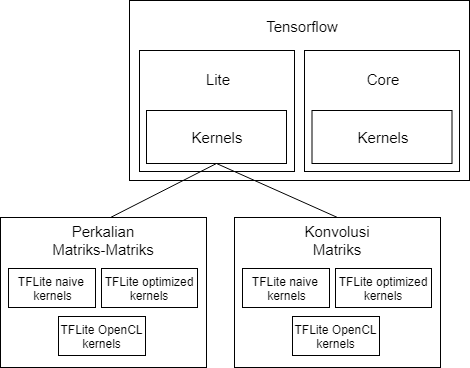
\includegraphics[width=0.75\textwidth]
	{pics/modifieddiagram.png}
	\caption{Skema modifikasi kode sumber Tensorflow Lite dengan menambahkan satu jenis \textit{kernel} baru untuk operasi perkalian matriks-matriks dan konvolusi matriks yang diimplementasikan melalui OpenCL dan berjalan di GPU.}
	\label{fig:modifieddiagram}
\end{figure}

Persiapan-persiapan OpenCL seperti yang disebutkan pada Bagian 2.5 memerlukan cukup banyak waktu. Untuk mengurangi biaya persiapan yang mahal, beberapa persiapan tidak dilakukan pada setiap proses \textit{inference}, namun hanya dilakukan satu kali pada awal berjalannya aplikasi \textit{Deep Learning}. Hal ini dilakukan dengan cara meletakkan persiapan-persiapan tersebut pada \textit{interpreter} Tensorflow Lite. Persiapan tersebut hanya dilakukan ketika \textit{interpreter} akan melakukan \textit{node parsing} terhadap graf Tensorflow Lite. \textit{Node parsing} adalah proses dimana \textit{interpreter} membuat objek-objek \textit{node} berdasarkan graf masukan, termasuk di dalamnya adalah objek lapisan \textit{fully-connected} dan objek lapisan konvolusi. Objek-objek hasil dari persiapan OpenCL seperti \textit{context} dan \textit{buffer} kemudian dapat diberikan sebagai argumen ketika \textit{interpreter} melakukan \textit{parsing} terhadap \textit{node} lapisan \textit{fully-connected} dan lapisan konvolusi. Ketika proses \textit{inference} berlagsung, objek lapisan \textit{fully-connected} dan lapisan konvolusi pada Tensorflow Lite dapat menggunakan objek-objek OpenCL yang telah dipersiapkan di awal. 

Persiapan untuk OpenCL yang dilakukan pada awal berjalannya aplikasi adalah membuat \textit{context}, membuat \textit{command queue}, membuat \textit{kernel}, dan membuat \textit{buffer}. Persiapan yang tidak dapat dilakukan hanya satu kali adalah menyalin data masukan operasi matriks dari memori CPU ke memori GPU. Proses menyalin data ini harus selalu dikerjakan pada setiap proses \textit{inference} karena data masukan bersifat dinamis. Perhatikan \pic~\ref{fig:initcl} dan \pic~\ref{fig:copydata} untuk mengetahui lebih jelas bagaimana persiapan untuk OpenCL dilakukan pada penelitian ini.

\begin{figure}
	\centering
	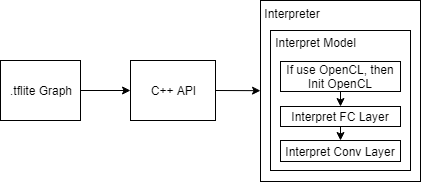
\includegraphics[width=0.75\textwidth]
	{pics/initcl.png}
	\caption{Ilustrasi persiapan untuk OpenCL yang dilakukan hanya satu kali di awal berjalannya suatu aplikasi \textit{Deep Learning}.}
	\label{fig:initcl}
\end{figure}

\begin{figure}
	\centering
	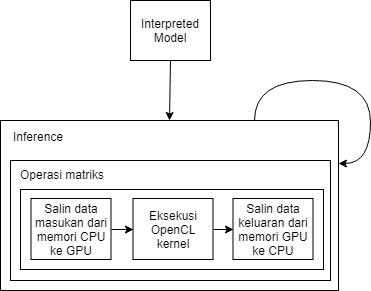
\includegraphics[width=0.75\textwidth]
	{pics/copydata.png}
	\caption{Ilustrasi proses transfer data antara memori CPU dan GPU yang dilakukan pada setiap proses \textit{inference}.}
	\label{fig:copydata}
\end{figure}

\section{Metode Eksperimen }
%-----------------------------------------------------------------------------%
Eksperimen dilakukan terhadap masing-masing jenis Tensorflow Lite \textit{kernel} untuk operasi perkalian matriks-matriks dan konvolusi matriks, yaitu Tensorflow Lite \textit{naive kernel} yang berjalan di CPU, Tensorflow Lite \textit{optimized kernel} yang berjalan di CPU, dan Tensorflow Lite OpenCL \textit{kernel} yang berjalan di GPU. Dalam eksperimen ini penulis mengukur kecepatan eksekusi tiga \textit{kernel} tersebut pada berbagai kasus ukuran matriks masukan. Hasil pengukuran kecepatan dari masing-masing \textit{kernel} kemudian dibandingkan. Untuk OpenCL \textit{kernel}, penulis melakukan dua jenis pengukuran kecepatan. Pertama, pengukuran dilakukan terhadap eksekusi OpenCL \textit{kernel} saja, tidak termasuk transfer data antara memori CPU dan GPU. Kedua, pengukuran dilakukan terhadap OpenCL \textit{kernel} beserta transfer data antara memori CPU dan GPU. Dengan demikian, penulis dapat mengetahui apakah \textit{bottleneck} dari program OpenCL yang telah diimplementasikan terletak terletak pada transfer data antar memori atau terletak pada eksekusi OpenCL \textit{kernel}. Untuk menghitung kecepatan dari suatu Tensorflow Lite \textit{kernel} penulis menggunakan \textit{wall-clock time} dengan cara menghitung selisih dari \textit{wall-clock time} sebelum dan sesudah Tensorflow Lite \textit{kernel} berjalan.